%\documentclass[french, a4paper, 12pt, titlepage]{article}
\documentclass[french, a4paper, 10pt]{article} % si la table des matiï¿œes est petite
\usepackage[utf8]{inputenc}
%\usepackage[latin1]{inputenc}
\usepackage[french]{babel}
% Modification des marges ------------------------------
\oddsidemargin -4mm 	% Marge de gauche -4mm
\textwidth 17cm 	% Largeur de gauche = 17cm
\textheight 22cm 	% Hauteur du texte = 22cm
\parindent 0cm		% Pas d'indentation de paragraphe
% -----------------------------------------------------
\usepackage[T1]{fontenc}
\usepackage{graphicx,color, caption}
\usepackage{epsfig}
\usepackage{fancyhdr}
%\usepackage{fancyvrb}
\usepackage{textcomp}
\pagestyle{fancy}
\usepackage{listings}		% pour incorporer des sources
\usepackage[francais]{layout}	% pour obtenir le layout
\usepackage{fullpage}		% pour obtenir le layout
\usepackage{makeidx}		% pour créer une table d'index
%\usepackage{shadow}		% pour faire des encadrements
\pdfminorversion=7
\begin{document}
% Titres sur  chaque page -----------------------------
\lhead{ } % Haut gauche
%\chead{Haut centre}
\rhead{Stéganographie : Bitmap et GIF}
\lfoot{\copyright{Foud Hind et Patti Philippe}}
\cfoot{ } % Bas centre - obligatoire !
\rfoot{\thepage} % Bas droite
\renewcommand{\headrulewidth}{0.4pt} 
\renewcommand{\footrulewidth}{0.4pt} 
% Numérotation et table des matières -----------------
\setcounter{tocdepth}{1}    % fixe la profondeur de la table des matières
\setcounter{secnumdepth}{5} % fixe la profondeur de la numérotation des sections et paragraph
% Page de garde --------------------------------------
\title{\emph{\textbf{Stéganographie : Bitmap et GIF}}}
\author{Foud Hind et Patti Philippe}
\date{3 avril 2020}
\maketitle
\tableofcontents
% Inclusion des textes
\section{Introduction}
L'objectif du projet est d'implémenter un programme illustrant le concept de sécurité suivant : la stéganographie.\\

Abordée du point de vue du cours de système, elle nous permet d'approfondir nos connaissances sur l'utilisation de la mémoire
pour stocker des informations.\\

Il est évident que pour mener à bien un projet de cette envergure, d'autres compétences nous ont été nécessaires
telles que l'apprentissage approfondi du langage C, notamment pour réaliser des opérations de manipulation de bits.
Nous avons également eu besoin d'apprendre en détails les structures de fichier bitmap et GIF, pour décider de la meilleure technique à
utiliser afin d'y cacher des messages.\\

Dans ce rapport, nous passerons en revue l'organisation du projet, le choix pour chaque format et la technique utilisée. 
Nous fournirons aussi un guide pratique pour utiliser les exécutables. 

\vspace{1.5cm}

\newpage
\section{Organisation du projet}
La structure de notre projet s'organise essentiellement en quatre répertoires dont voici le détail :\\ 

\begin{itemize}
    \item \textbf{dist :} contient les exécutables du programme dans un dossier bmp et gif respectifs.
    \item \textbf{rapport :} contient le rapport en format tex et pdf, les fichiers qui serviront à construire celui-ci 
    ainsi que le makefile qui le lancera. On pourra également y trouver le document pdf de la présentation.
    \item \textbf{rsc :} contient les ressources qui servent d'input au programme [bitmap et gif] ainsi que les outputs 
    qui seront produits dans un dossier bmp et 
    gif respectifs.
    \item \textbf{src :} contient les sources du programme dans un dossier bmp et gif respectifs\\
\end{itemize}
On peut également trouver à la racine, un makefile général qui automatise le lancement du programme ainsi qu'un fichier README.

\vspace{1.5cm}
\section{Guide pratique}
\lstinputlisting[language=make, firstline=1, lastline=18]{../makefile}

\newpage
\section{Stéganographie : Définition}
La stéganographie est l'art de la dissimulation : son objet est de faire passer inaperçu des données dans d'autres données. 
Elle se distingue de la cryptographie, « art du secret », qui cherche à rendre un message inintelligible à autre que qui-de-droit.\\
Les fichiers peuvent être de type divers : fichiers image, audio, html, vidéos etc.\\
Parmi les scénarios de tests envisagés, nous avons tenté de cacher :\\

\begin{itemize}[label=$\diamond$, font=\LARGE \color{black}]
    \item un \textbf{texte} (.txt, .pdf) dans une \textbf{image} (.bmp/.gif)
    \item une \textbf{image} (.bmp, .gif) dans une \textbf{image} (.bmp/.gif)
    \item une \textbf{vidéo} (.mp4) dans une \textbf{image} (.bmp/.gif)\\
\end{itemize}

Il est évident que pour que cela soit possible, des conditions sont à poser.
Il faudra bien sûr que le fichier à cacher soit plus petit que le fichier objet. Il faudra aussi peauffiner les conditions de 
faisabilité qui sont fortement dépendantes du type de fichier et veiller à respecter la règle d'or : le dissimuler à tout prix.
Cela signifie qu'il faudra limiter au maximum l'impact sur le fichier dans lequel on aura caché des données sinon ce serait contraire
au principe de stéganographie.

\vspace{1.5cm}
\begin{center}
    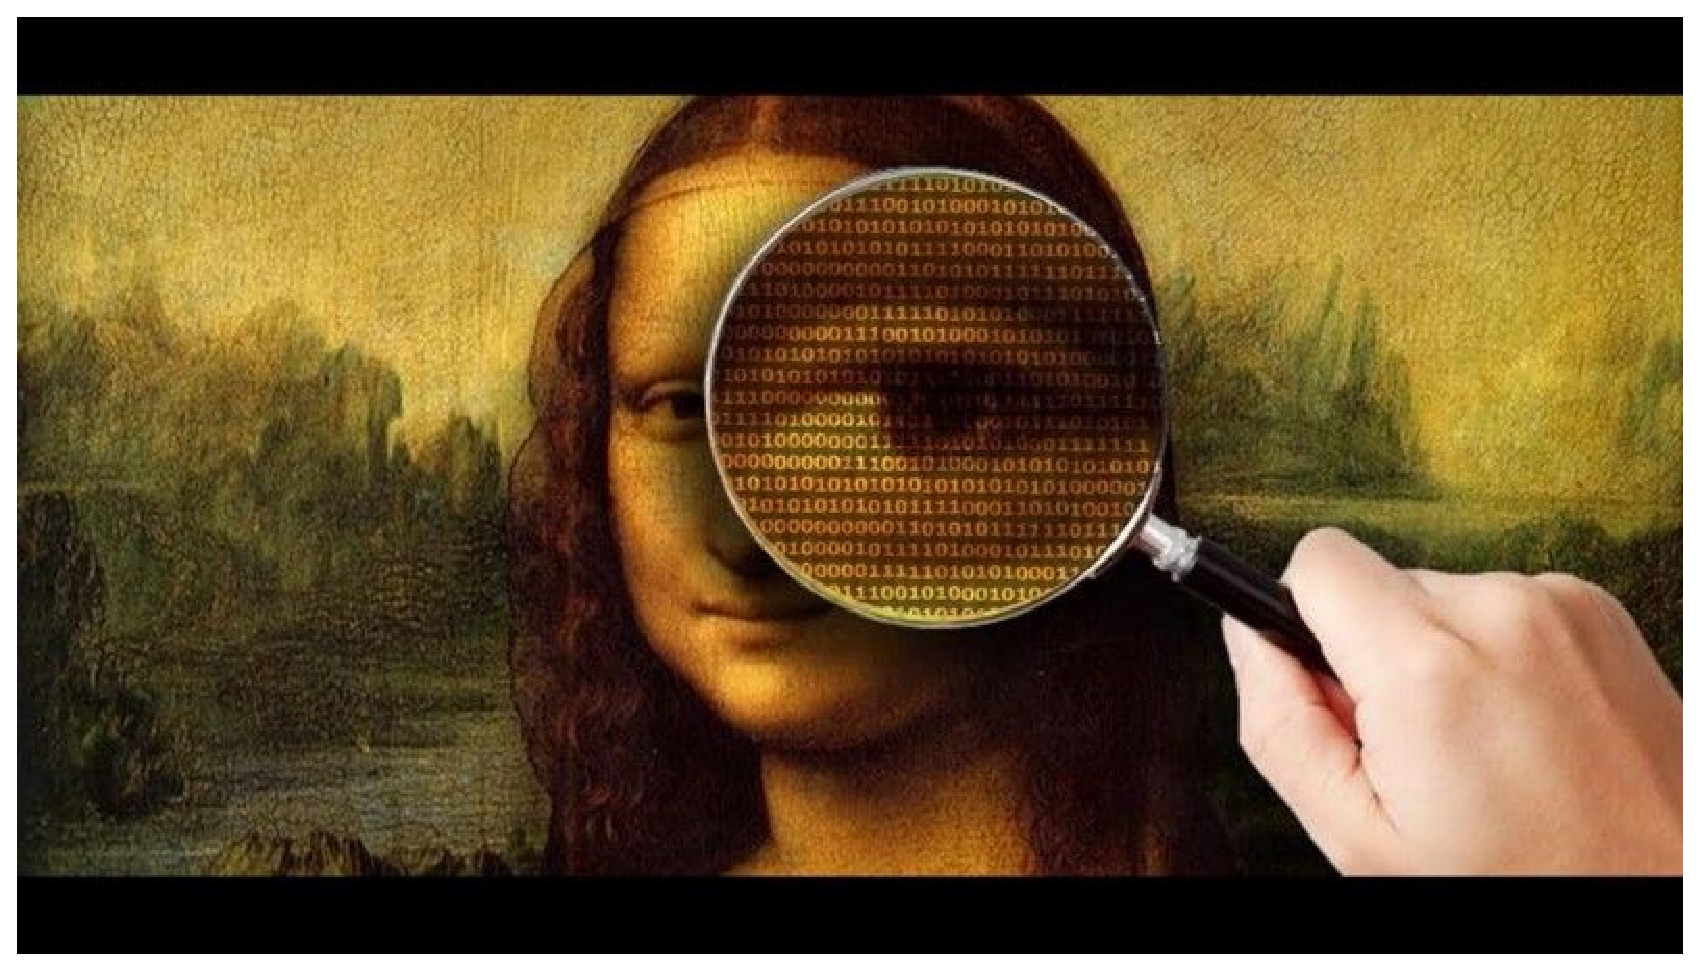
\includegraphics[width=10cm]{steganographie.eps}
\end{center}

\newpage
\section{Least Significant Bit (L.S.B.)}
Pour coder/décoder un message, nous employons la technique du Least Significant Bit (LSB). \\
Comme vous le voyez sur le schéma ci-dessous [Schéma général], cette technique consiste à se focaliser sur le bit le moins 
important d'un byte appelé le bit de poids faible.
Pour coder le message, il suffit de lire un byte à cacher et de l'encoder dans le bit de poids faible d'un byte choisi.
Pour décoder le message, il suffit de lire le bit de poids faible de ces bytes 'élus' et de reformer un message compréhensible.\\\\

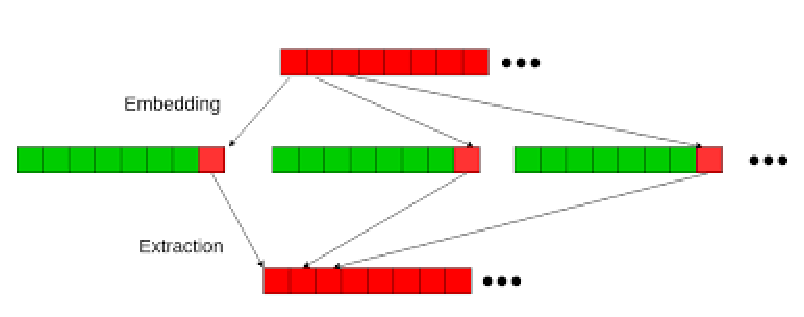
\includegraphics[width=15cm]{lsb.eps}\\

C'est cette logique que nous nous sommes employés à suivre dans le cas de traitement sur ces deux formats de fichiers image.
Ainsi, la technique est la même mais certains choix se sont imposés de part les différences entre les deux structures de ces 
fichiers image. Ces choix portent notamment sur 'l'élection' des bytes dans lesquels nous allons cacher l'information.
En effet, pour que le message ait le plus petit impact possible sur le fichier image, il faut employer des bytes qui peuvent
perdre un bit d'information sans que cela ne se remarque.
Par exemple, pour une couleur codée en rgb, le changement du dernier bit a un impact très faible, quasi invisible à l'oeil nu.
Il est donc adéquat pour y dissimuler des données.\\\\

\newpage
\subsection{Encodage : extrait de code source concernant la manipulation des LSB}
\lstinputlisting[language=c, firstline=57, lastline=72]{../src/utils/bmp.c}

\subsection{Décodage : extrait de code source concernant la manipulation des LSB}
\lstinputlisting[language=c, firstline=30, lastline=47]{../src/utils/bmp.c}
\lstinputlisting[language=c, firstline=92, lastline=95]{../src/utils/bmp.c}


\section{Bitmap}

\subsection{Aperçu du Bitmap}
Le format BITMAP aussi appelé DIB (Device Independent Bitmap) a été conçu par Windows corporation pour pouvoir échanger des images entre devices sans avoir à se soucier de la logique de ceux-ci.
Ces images ont des extensions .bmp ou encore .dib.\\
Une image bitmap est un format de fichier généralement non compressé. Cela signifie que chaque pixel possède sa représentation sous forme d'une série de bits.
Les bitmaps n'ont aucune perte de données et sont donc généralement plus lourds.
On peut opposer leur structure à celle d'une image PNG, JPEG ou encore GIF, qui utilisent la compression pour regrouper des pixels similaires.\\
Les headers des bitmaps peuvent employer plusieurs versions. Ces versions donnent plus ou moins de métadonnées sur le bitmap. 
Le BITMAPINFOHEADER est une des versions les plus simples et rétrocompatible. 
Actuellement, il existe des versions plus complètes, tels que le BITMAPV4HEADER ou BITMAPV5HEADER.\\
La structure du format BITMAP est connue et disponible en ligne. En voici un schéma, utilisant le BITMAPINFOHEADER :\\

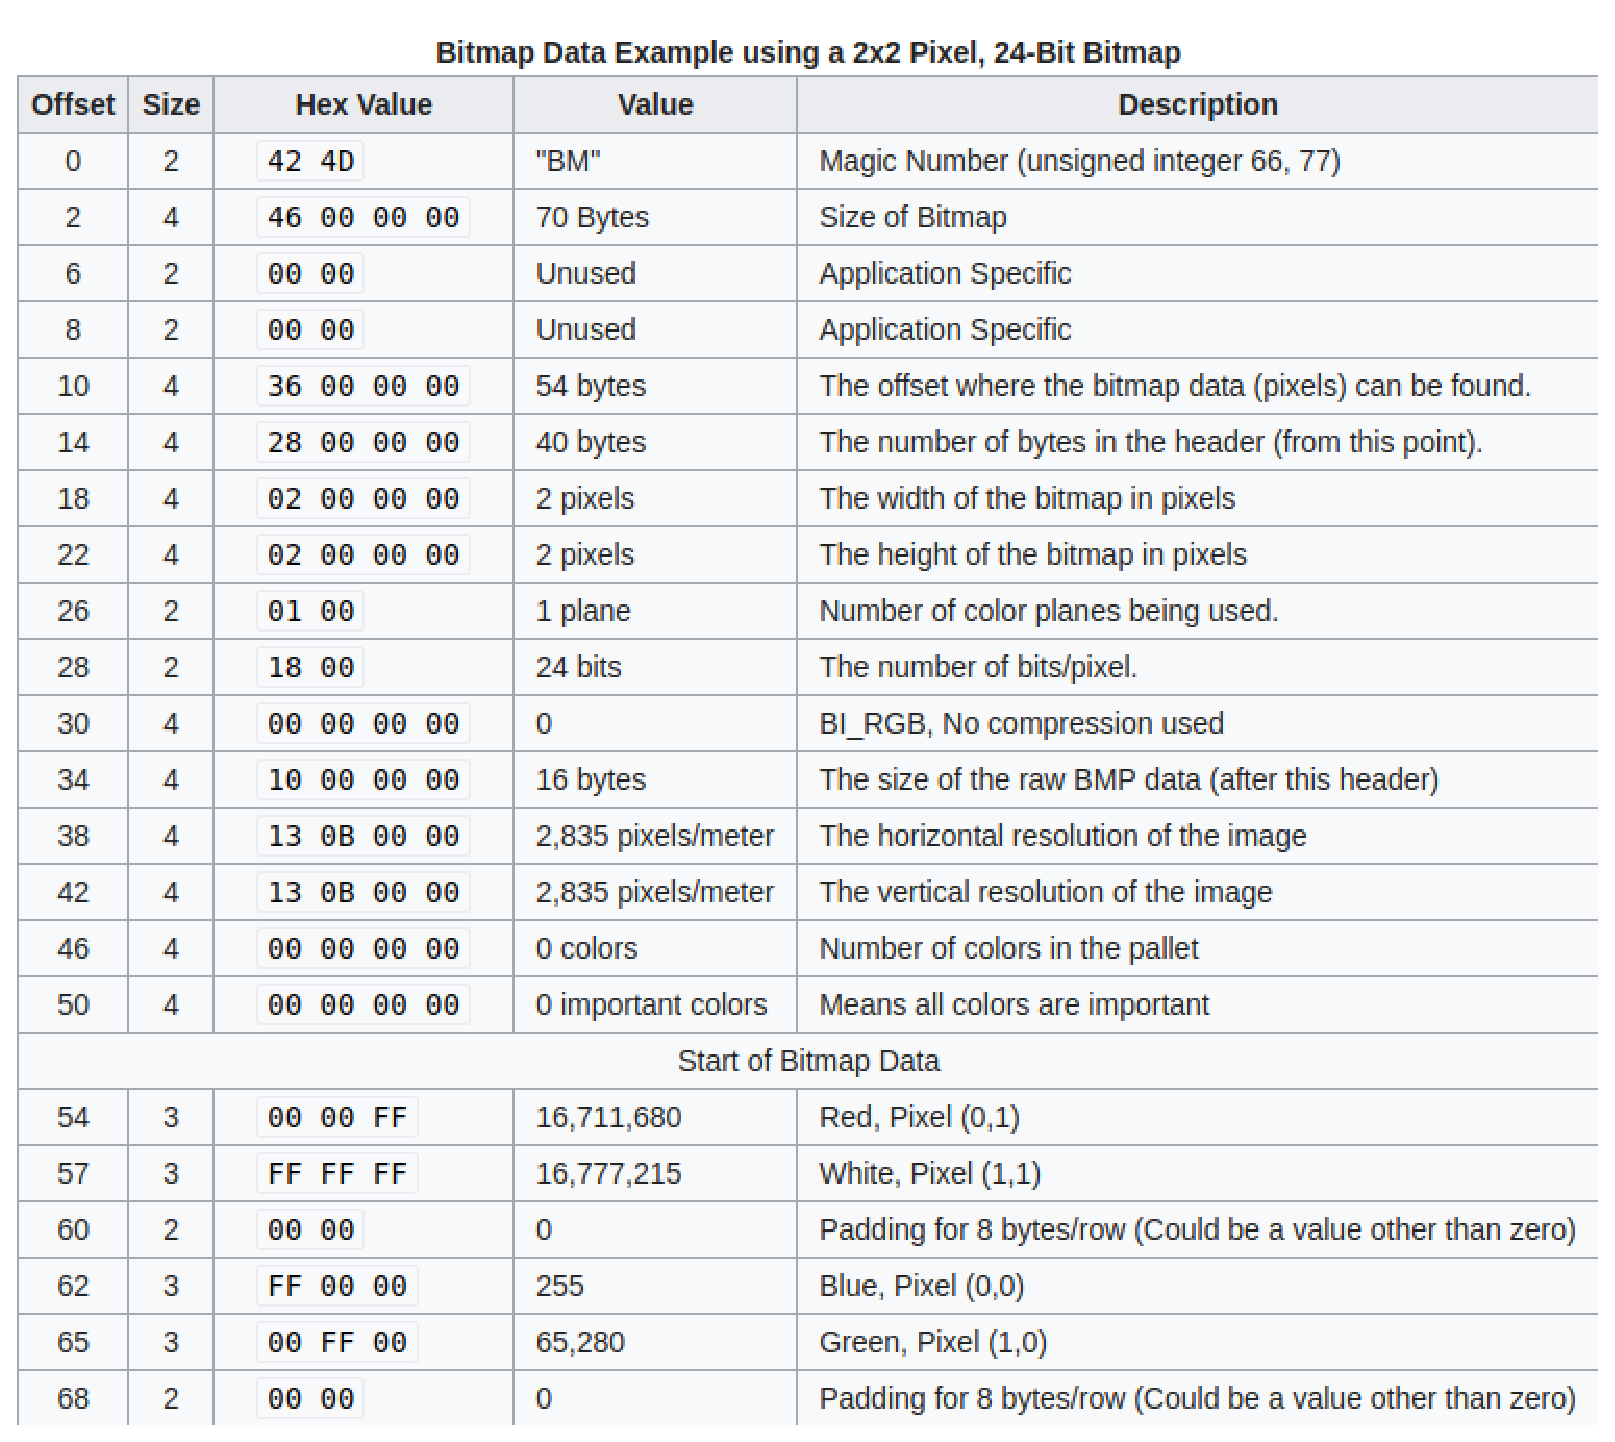
\includegraphics[width=14cm]{bitmap_structure.eps}

\subsection{Application du LSB}
Nous cachons les données dans les bytes décrivant les couleurs de l'image source, juste après le header.
Les modifications étant faites sur des couleurs, l'image est peu altérée. Les modifications sont invisibles à l'oeil humain.
De plus, ce fichier n'utilisant généralement pas d'algorithme de compression, on ne doit pas se soucier de perte de données, 
ce qui aurait probablement impacter le décodage d'une image dans laquelle on aurait caché des données.

\vspace{1.5cm}
 % pas de saut de page
\section {GIF}
\subsection {Pourquoi le GIF?}
Le format GIF permet de stocker plusieurs images dans un fichier. Ceci permet de créer des diaporamas, voire des animations si les images sont affichées à un rythme suffisamment soutenu. Chaque image d'une animation peut avoir sa propre palette.
Le GIF est un format très utilisé, particulièrement sur les réseaux sociaux. Ce projet peut donc intéressé pas mal de gens. \\\\
La structure du format GIF est connue et disponible en ligne. En voici un schéma : \\\\
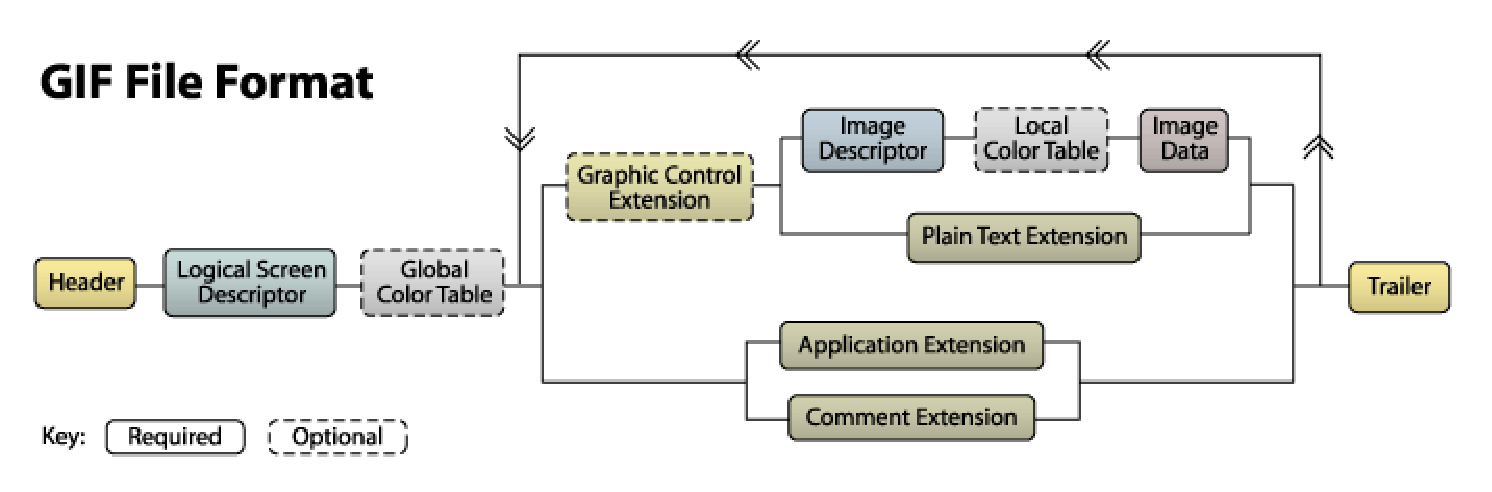
\includegraphics[width=15cm]{gif_structure.eps}
\subsection {Application du LSB}
Nous avons choisi de cacher des informations dans les couleurs qui se trouvent dans les Local Color Table. Cette section facultative peut revenir devant chaque bloc image data. Si cette section n'existe pas, nous la rajoutons.\\\\
Il est possible de calculer la taille maximale du message cachée à l'avance, en comptant le nombre de bloc image data et en le multipliant par le nombre de byte dans la Global Color Table.
\subsection {Avancement}
\subsubsection {Lecture}
Le programme peut déja lire un gif en entier, section par section. Les tailles des sections sont indiquées à des endroits différents par sections. La lecture se fait donc différemment en fonction de la section.\\\\
De plus, on peut déja savoir le nombre maximal de Local Color Table pour le fichier modifié.
\subsubsection {Lecture}
Le programme réécrit le gif dans un nouveau fichier, en insérant des Local Color Table, identique à la Global Color Table. Ceci permettra d'y insérer un message. L'insertion du message devrait être évidente, vue qu'elle sera presque identique à la stéganographie dans un fichier bitmap.\\\\
Il y a toutefois encore un bug dans la réécriture du fichier gif, probablement à l'écriture des nouvelles Local Color Table.
\subsection {Guide pratique}
Pour exécuter le projet actuel, exécuter le makefile à la racine du fichier.
Voici quelques options possibles avec le makefile : \\
\lstinputlisting[language=make, firstline=1, lastline=18]{../makefile}
\newpage
%
%
%
%
\section {exemples latex}
Vous découpez votre travail en chapitre (section), en sous-chapitre (subsection) et en sous-sous-chapitre (subsubsection)
Il suffit de taper le texte au kilomètre. \emph{Il est possible d'insister} sur un passage.
Vous appelez la commande :
\lstset{frame=trBL}
\begin{lstlisting}
aspell -t - -encoding='iso8859-15' -c VotreFichier.tex
\end{lstlisting}
\subsubsection {Une énumération}
Si vous devez utiliser des puces :
\begin{itemize}
\item point 1
\item point 2
\end{itemize}
Si vous devez énumérer :
\begin{enumerate}
\item point 1
\item point 2
\end{enumerate}
Vous pouvez mélanger à autant de niveaux que vous le souhaitez.
\subsubsection{Un tableau}
\begin{tabular}{|l|l||c||r|} %left ou r ou c ou p[dimension]
\hline
Jour & Heures & Local & Cours \\
\hline
Mardi    &  3..4  & 503 & Système\\
Mardi    &  5..8  & 503 & Sécurité\\
\hline
Mercredi  &  1..2  &  201 & Assembleur\\
Mercredi  &  3..4  &  003 & Labo assembleur\\
\hline
\end{tabular}
\subsubsection {Intégrer une source}
Pour énumérer une source, vous pouvez préciser ce que vous souhaitez avec lstset. 
\lstset{language={},frame=trBL}
\begin{lstlisting}
MOV EAX,10 ; place 10 dans le registre EAX
ADD EAX,20 ; ajoute 20 au contenu de EAX
\end{lstlisting}
\subsubsection {Intégrer un graphique}
Vous pouvez intégrer un graphique mais il faut qu'il soit en format eps.\\
Vous pouvez dessiner avec l'outil oodraw qui permet d'exporter votre dessin dans ce format eps.\\
Vous pouvez transformer un jpeg en eps avec l'outil sam2p ou convert qui se trouve dans le package ImageMagick\\
%\includegraphics[width=8cm]{Dessin.eps}
\subsubsection {Mode mathématique}
C'est un des points forts de latex qui permet d'écrire des formules mais aussi des caractères spéciaux tels que :
$2^{32} \approx 10^{9}$ car $\log{_{10}}{2} \approx 0.3$ et $32*0.3 \approx 9$.
\subsubsection {Quelques trucs faciles}
\begin{itemize}
\item \verb+\\+ permet de passer à la ligne suivante.
\item \verb+\\[2cm]+ permet de passer à la ligne suivante + une tabulation verticale de 2cm. Sont autorisés mm, cm et pts.
\item \verb+\newpage+ permet de forcer un passage à la page suivante.
\end{itemize}
\subsubsection {Compiler le texte}
Un script permet d'automatiser cette compilation:
\begin{lstlisting}
#! /bin/sh
FN=Mrapport # Le nom du document.
latex $FN.tex
latex $FN.tex # 2 passages pour la TOC
rm $FN.aux $FN.log $FN.out
dvips $FN.dvi -o $FN.ps
rm $FN.dvi
gv $FN.ps # pour visualiser et imprimer
\end{lstlisting}
%-----------------------------------------------------------------------------------
\subsection{Conclusions}
Ce travail montre, qu'en quelques minutes, on peut déjà fournir un travail présenté de façon professionnelle, lisible par tous et dans un format standard.
Pour ne pas avoir de soucis, les commandes à utiliser pour obtenir un document postcript sont latex et dvips, il ne faut jamais utiliser pdflatex. 

Ce document peut être encore complété avec d'autres exemples qui seraient utiles. Ces nouveaux exemples pourraient être intégrés dans le premier ou un deuxième chapitre. Ceci, sans oublier qu'il s'agit d'un document utile pour commencer très rapidement à écrire en latex et non un mode d'emploi complet de latex qui serait obligatoirement très volumineux.
%-----------------------------------------------------------------------------------
\subsection{Références}
\begin{itemize}
\item http://www.grappa.univ-lille3.fr/FAQ-LaTeX/ 
\item http://tex.loria.fr/
\item http://tex.loria.fr/english/packages.html
\end{itemize}
%-----------------------------------------------------------------------------------
\subsection{Annexes }
Vous trouvez dans le casier, un répertoire LATEX contenant :
\begin{itemize}
\item Mrapport.tex : le document latex maître
\item LatexSimple.tex : ce document latex
\item dessin.odg et dessin.eps : le dessin intégré dans le texte
\item go : un script qui permet de compiler rapport.tex, sans argument.
\end{itemize}
%-----------------------------------------------------------------------------------

\section {Conclusion}
Ce projet nous a permis de pratiquer de nombreuses compétences importantes pour les futurs informaticiens que nous sommes
telles que le travail de recherche et la collaboration.\\

Nous avons dû appronfondir nos connaissances en programmation C pour répondre à des besoins de compréhension des formats 
de fichier mais aussi pour prendre les meilleures décisions concernant l'implémentation du code.
Dans un premier temps, nous nous sommes efforcés d'afficher les fichiers afin d'en maitriser les différentes sections
et contraintes qui y sont liées.\\

Nous avons ensuite commencé à coder selon une technique reconnue pour être simple et efficace qui se base sur le LSB évoquée
plus haut. Il s'agit donc de travailler sur les bits de poids faible ce qui crée une différence imperceptible à l'oeil humain.
D'abord dans le bitmap, pour des questions de simplicité, puis dans le gif.\\

Nous avons réutiliser le code le plus possible. 
Ce qui implique que le traitement est le même, la seule différence liée au format est l'endroit où l'on applique ce traitement.
Nous travaillons après le header dans le cas des bitmaps alors que pour les gifs, nous traitons les local color table.
Cela se justifie par le fait que celles-ci ne souffrent pas de compression et garantissent, en principe, un décodage sans encombres.\\

Pour terminer, nous avons également envisagé d'utiliser une autre technique appelée le MSB. 
Comme son nom l'indique, elle implique de travailler sur les bits de poids fort, ce qui trahit la manipulation du fichier. 
Ceci ne fait partie de notre implémentation que pour démontrer ce qu'il se passe lorqu'on ignore la bonne pratique.
 
\vspace {5cm}

\section {Références}
https://docs.microsoft.com/\\
https://www.fileformat.info/\\
http://www.matthewflickinger.com/lab/whatsinagif/\\
\printindex			% Impression de la table des index
\end{document}
